%%%%%%%%%%%%%%%%%%%%%%%%%%%%%%%%%%%%%%%%%%%
\fe{\section{Rappels}}{\section{Reminders}}
\label{rappels}
%%%%%%%%%%%%%%%%%%%%%%%%%%%%%%%%%%%%%%%%%%%

\begin{frame}{\fe{Cast3M, quid ?}{What is Cast3M?}}
  \begin{center}
    \fe{Logiciel de simulation utilisant la \g{méthode des éléments finis} en \g{mécanique/thermique} des \g{structures} et des \g{fluides}}
       {A simulation software using the \g{finite element method} in \g{thermal and mechanical} analysis of \g{structures} and \g{fluids}}\pause
  \end{center}
  \begin{itemize}
    \item \fe{Résolution d'\g{équations aux dérivées partielles}}
             {\g{Partial differential equations} solver}\pause
    \item \fe{\g{Système complet} : solveur, pré/post-processeur, visualisation, import/export des données\dots}
             {\g{Complete software}: solver, pre-processing and post-processing, visualization, reading/writing data\dots}\\~\\
    \begin{center}
      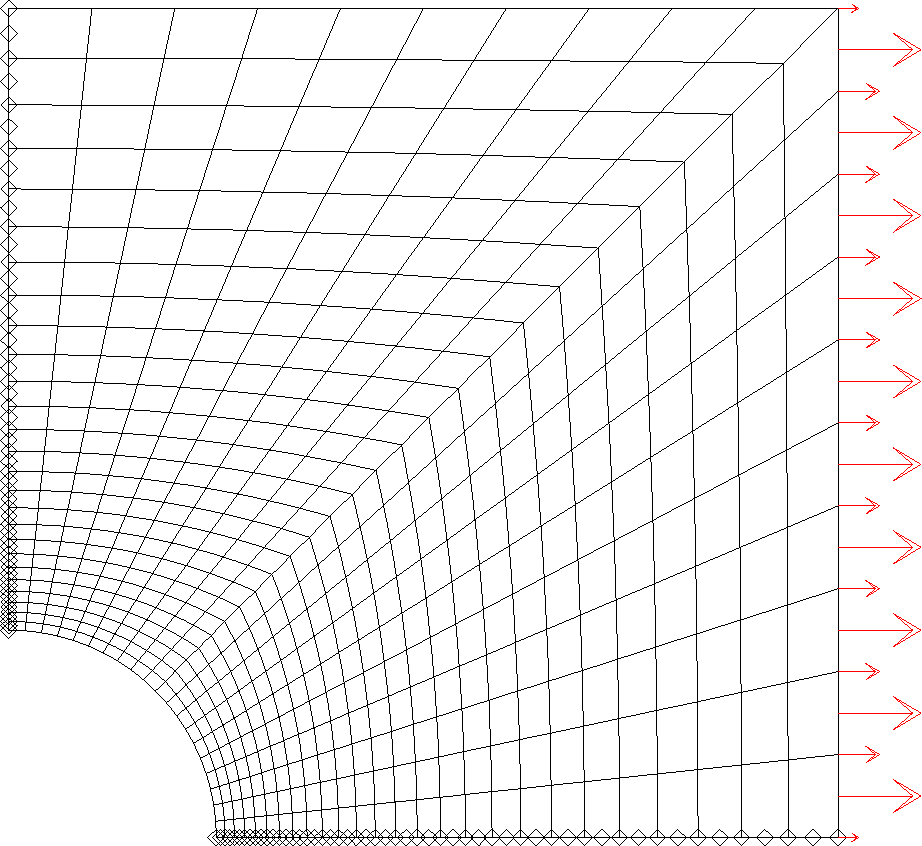
\includegraphics[height=0.25\textheight]{images/plaque.1} \:
      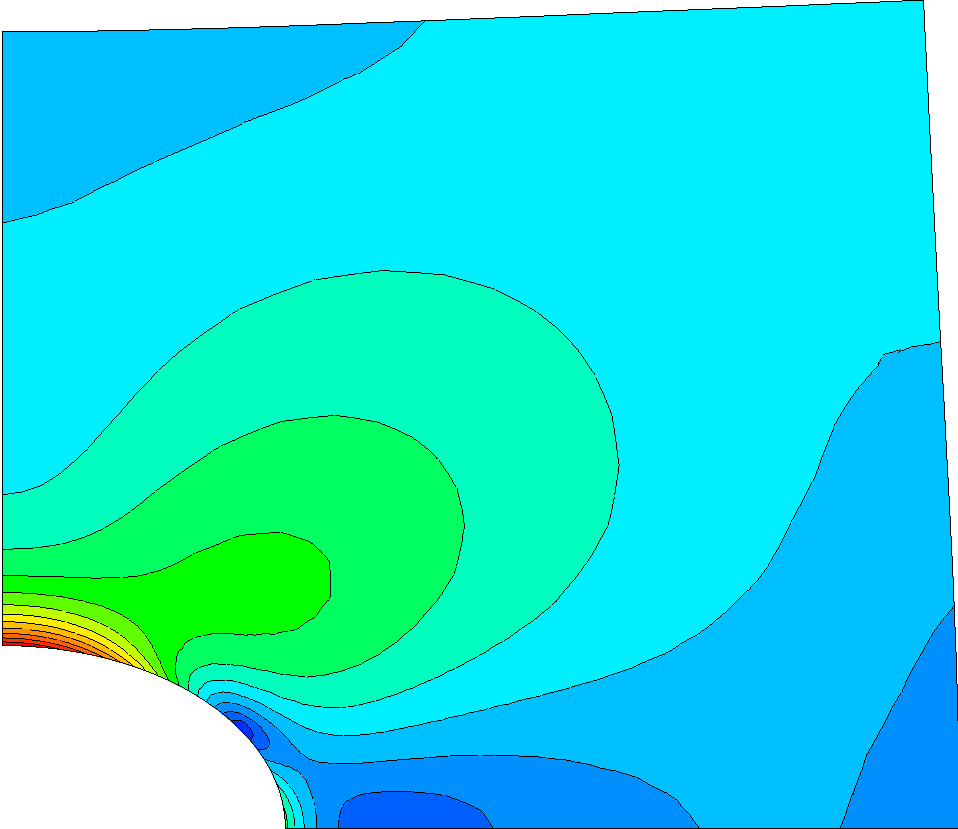
\includegraphics[height=0.25\textheight]{images/plaque.2} \:
      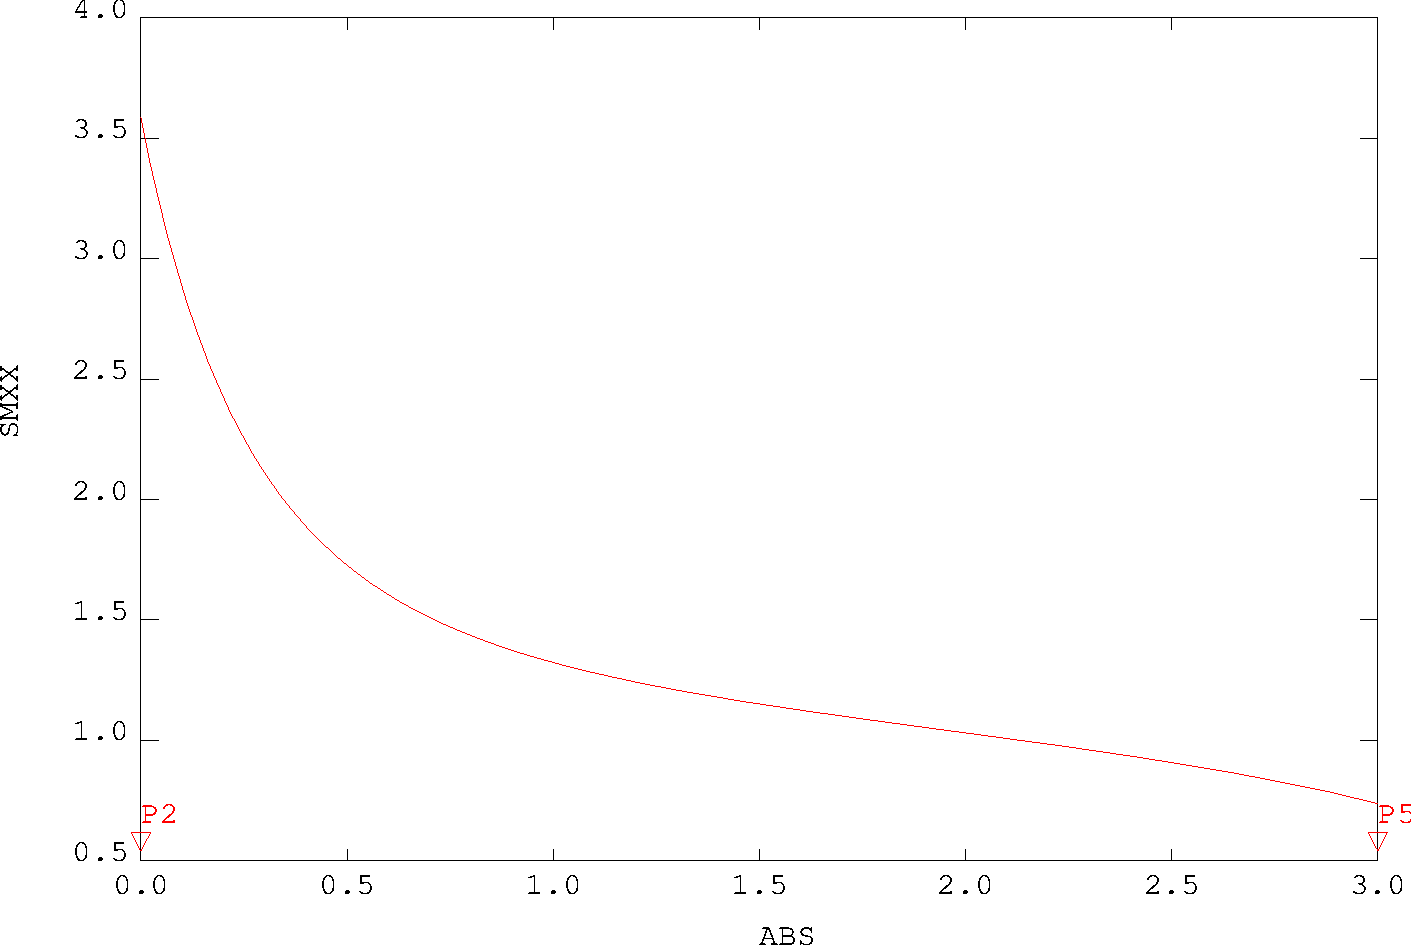
\includegraphics[height=0.25\textheight]{images/plaque.3}
    \end{center}\pause
    \item \fe{Basé sur un langage de commande : \g{Gibiane} (orienté objet)}
             {Based on a programming language: \g{Gibiane} (objet-oriented)}\\
  \end{itemize}
\end{frame}

\begin{frame}{\fe{Nombreux domaines d'application}{Wide range of applications}}
  \small{
  \begin{itemize}
    \item<1->\fe{\g{Mécanique des structures}}{\g{Structural mechanics}}\\
    \footnotesize{
    \fe{\red{Quasi-statique} (non linéarités matériau, géométrie, conditions limites)}
       {\red{Quasi-static} (non linear behavior, geometry, boundary conditions)}\\
    \onslide<1>{
      \begin{textblock*}{5cm}(2cm,0.3cm)
        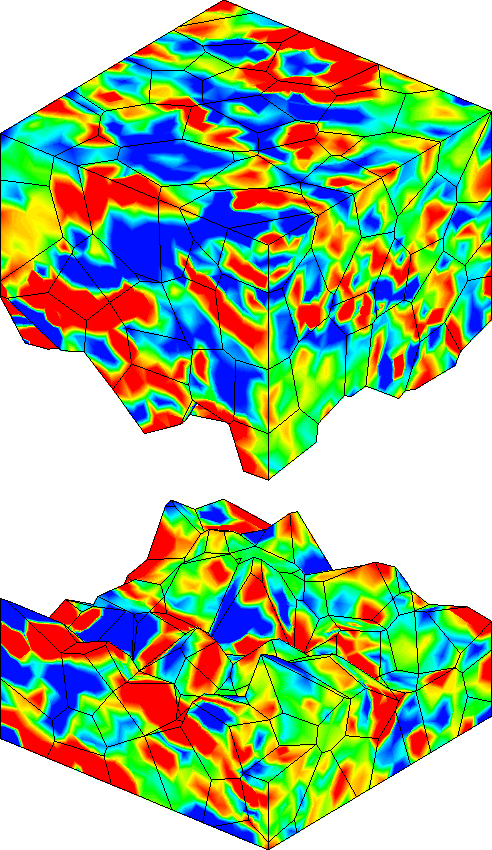
\includegraphics[height=0.4\textheight]{images/polycristal}
      \end{textblock*}
      \begin{textblock*}{5cm}(5cm,1.2cm)
        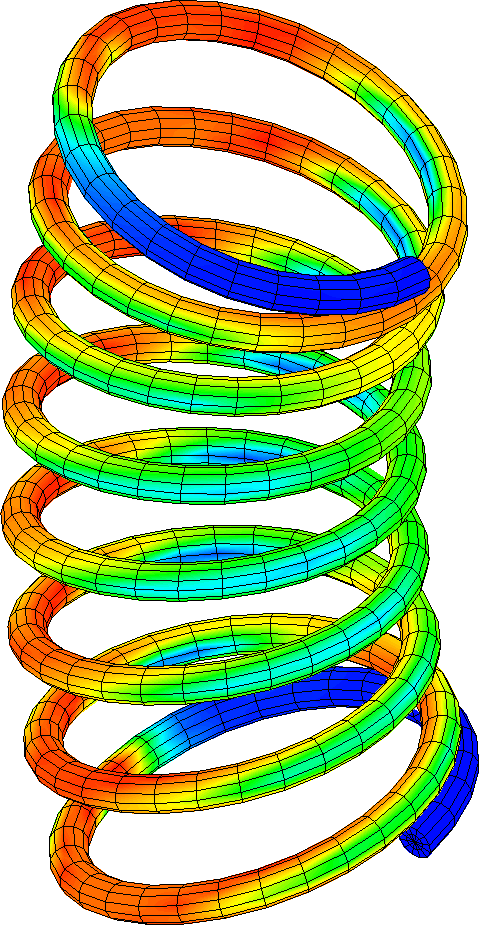
\includegraphics[height=0.4\textheight]{images/ressort}
      \end{textblock*}
      \begin{textblock*}{5cm}(8cm,2.1cm)
        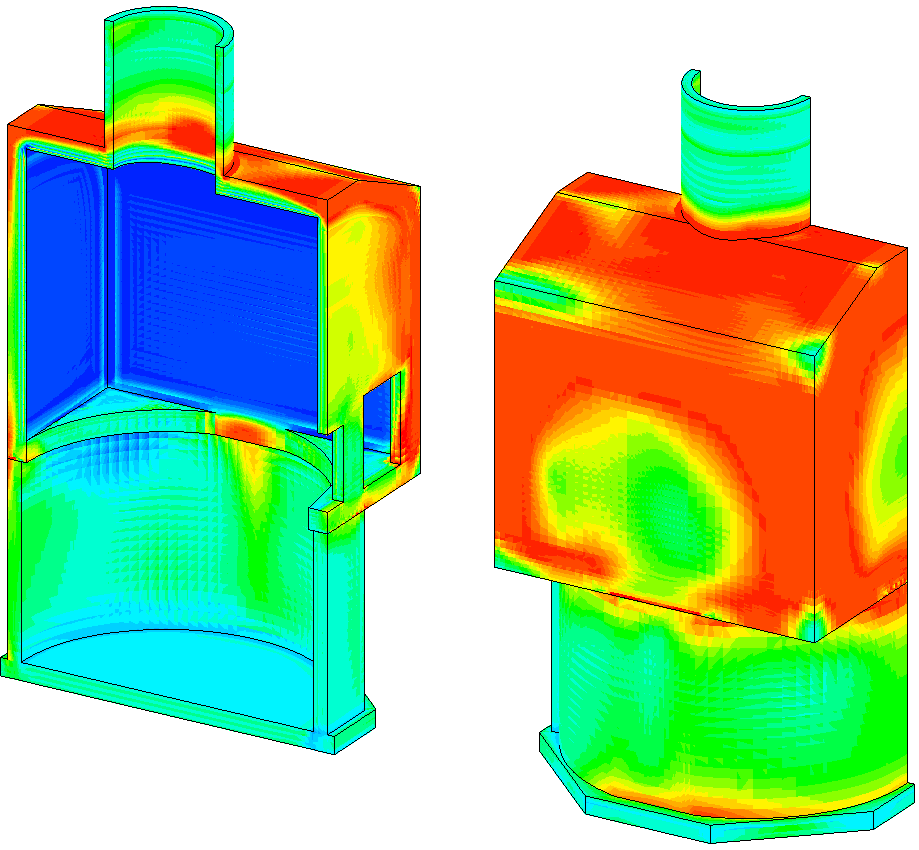
\includegraphics[height=0.4\textheight]{images/galatee}
      \end{textblock*}
      \begin{textblock*}{5cm}(9.4cm,5.6cm)
        \tiny{\emph{(S. Durand)}}
      \end{textblock*}}
    \onslide<2->\fe{\orange{Contact/frottement}, \green{Flambage}}
                    {\orange{Contact/friction}, \green{Buckling}}\\
    \onslide<2>{
      \begin{textblock*}{5cm}(1cm,0.3cm)
        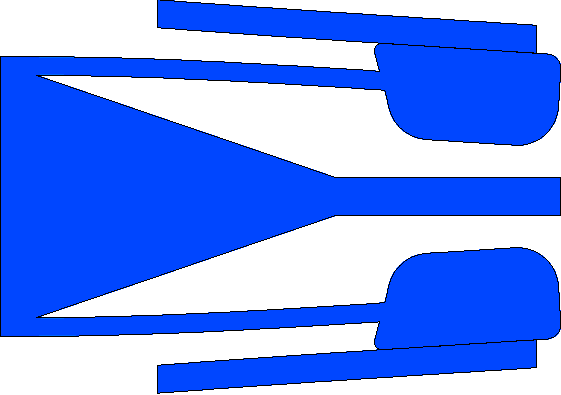
\includegraphics[height=0.25\textheight]{images/sac_a_dos.15}
      \end{textblock*}
      \begin{textblock*}{5cm}(4.8cm,0.3cm)
        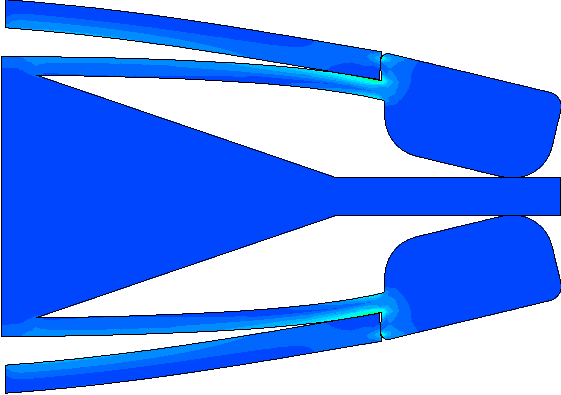
\includegraphics[height=0.25\textheight]{images/sac_a_dos.32}
      \end{textblock*}
    \begin{textblock*}{5cm}(8.5cm,0.3cm)
        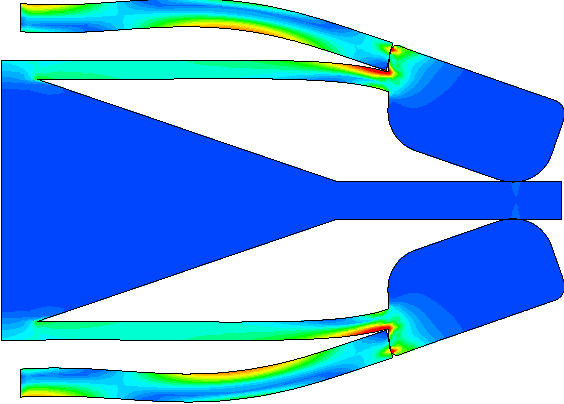
\includegraphics[height=0.25\textheight]{images/sac_a_dos.41}
      \end{textblock*}}
    \onslide<3->\fe{\blue{Dynamique} (temporelle, modale, interaction fluide structure)}
                    {\blue{Dynamic} (temporal, modal, fluid structure interaction)}\\
    \onslide<3>{
      \begin{textblock*}{5cm}(1cm,0.3cm)
        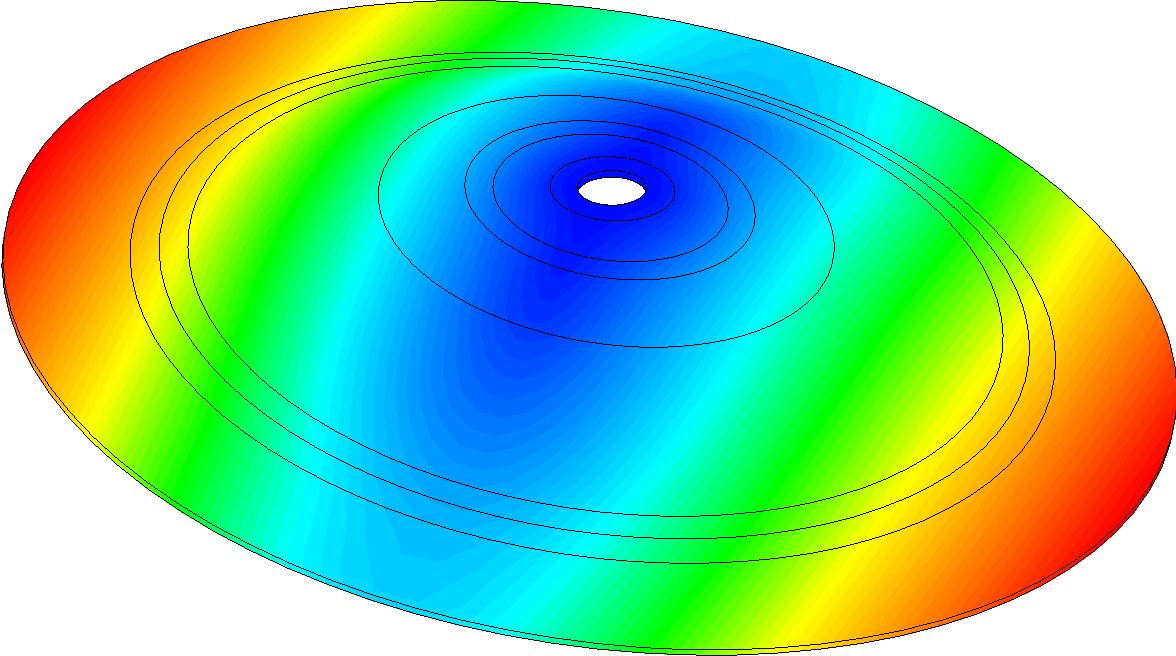
\includegraphics[height=0.2\textheight]{images/cymbale_mode_1}
      \end{textblock*}
      \begin{textblock*}{5cm}(4.8cm,0.3cm)
        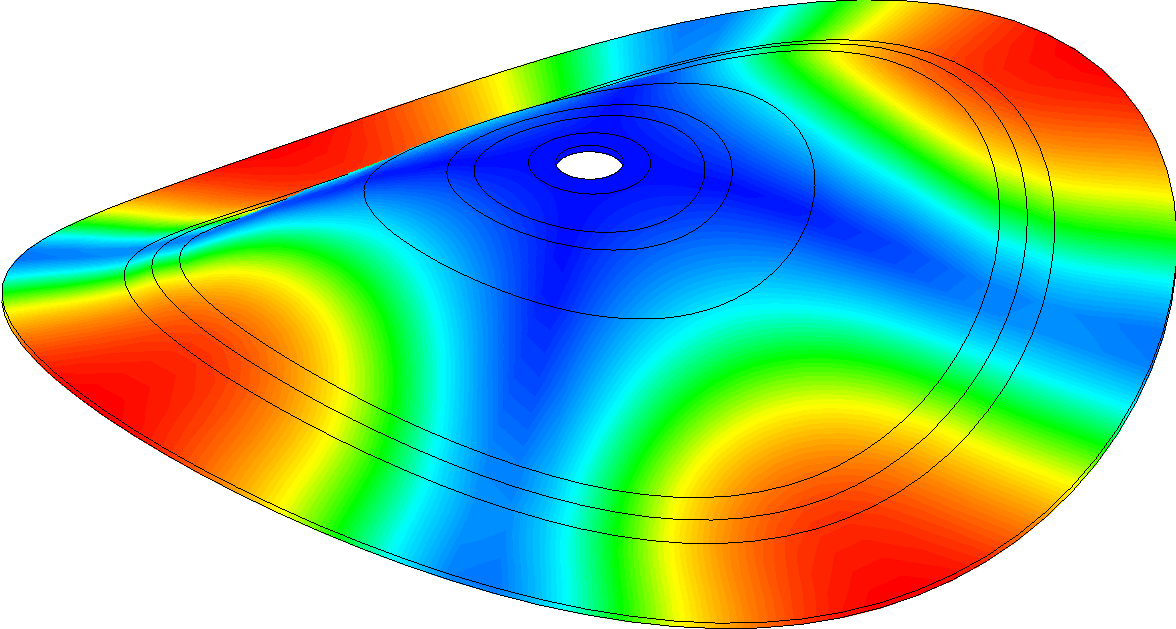
\includegraphics[height=0.2\textheight]{images/cymbale_mode_2}
      \end{textblock*}
      \begin{textblock*}{5cm}(8.5cm,0.3cm)
        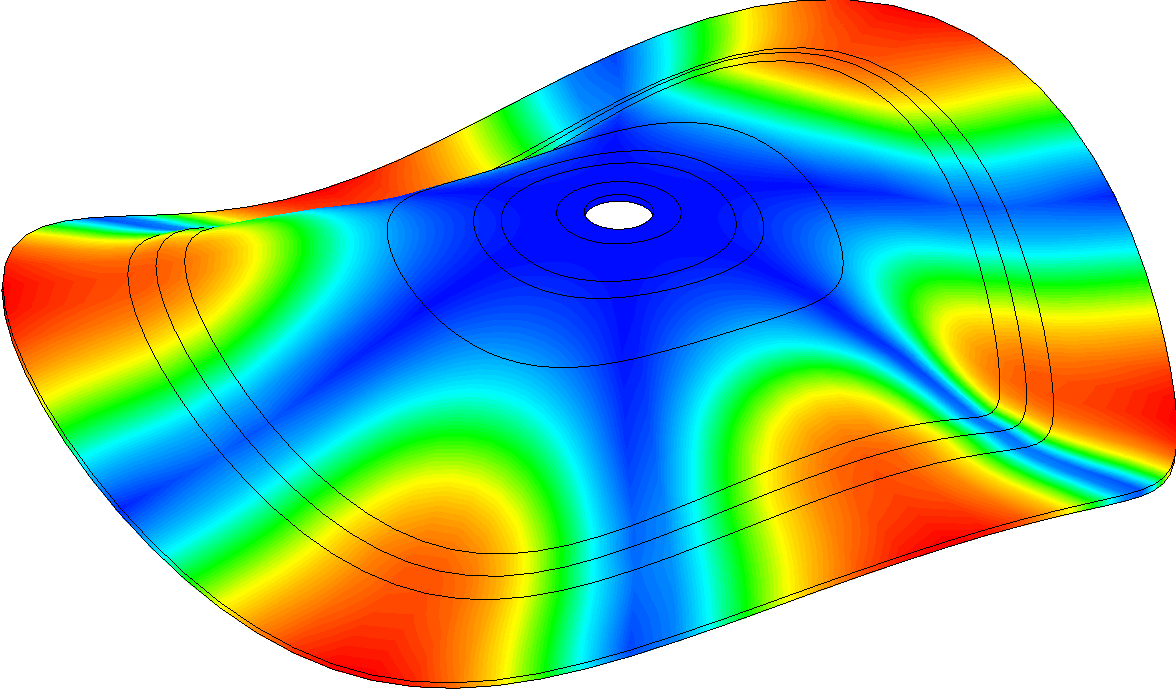
\includegraphics[height=0.2\textheight]{images/cymbale_mode_4}
      \end{textblock*}}
    \onslide<4->\fe{\violet{Rupture} (XFEM, propagation dynamique, zones cohésives)}
                   {\violet{Fracture} (XFEM, dynamic propagation, cohesive zones models)}\\
    \onslide<4>{
      \begin{textblock*}{12cm}(1.5cm,0.3cm)
        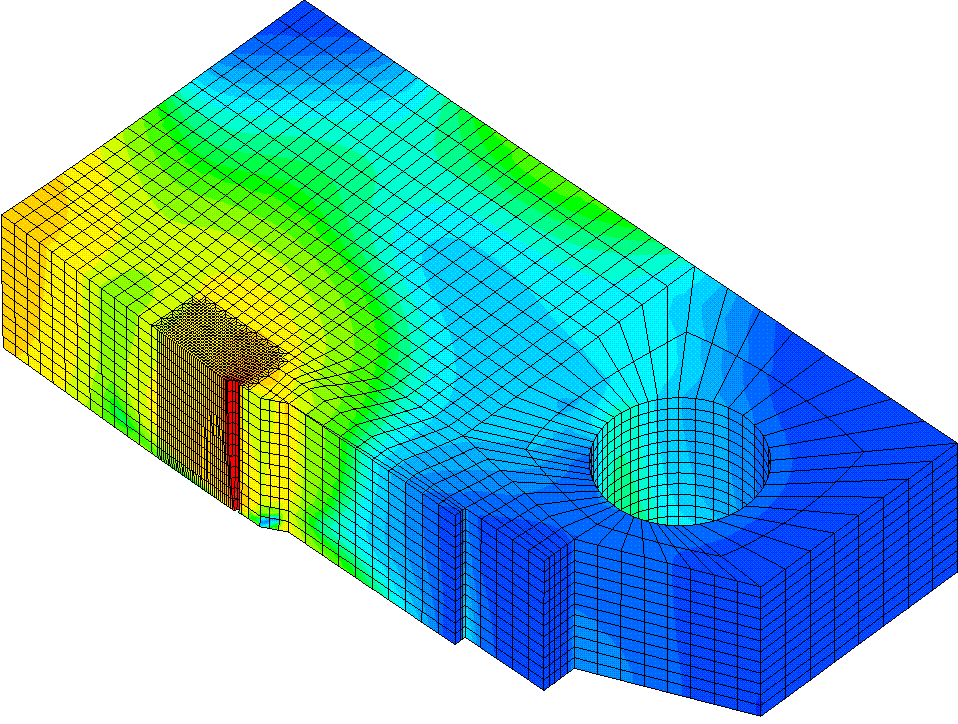
\includegraphics[height=0.25\textheight]{images/rousselier_03}
        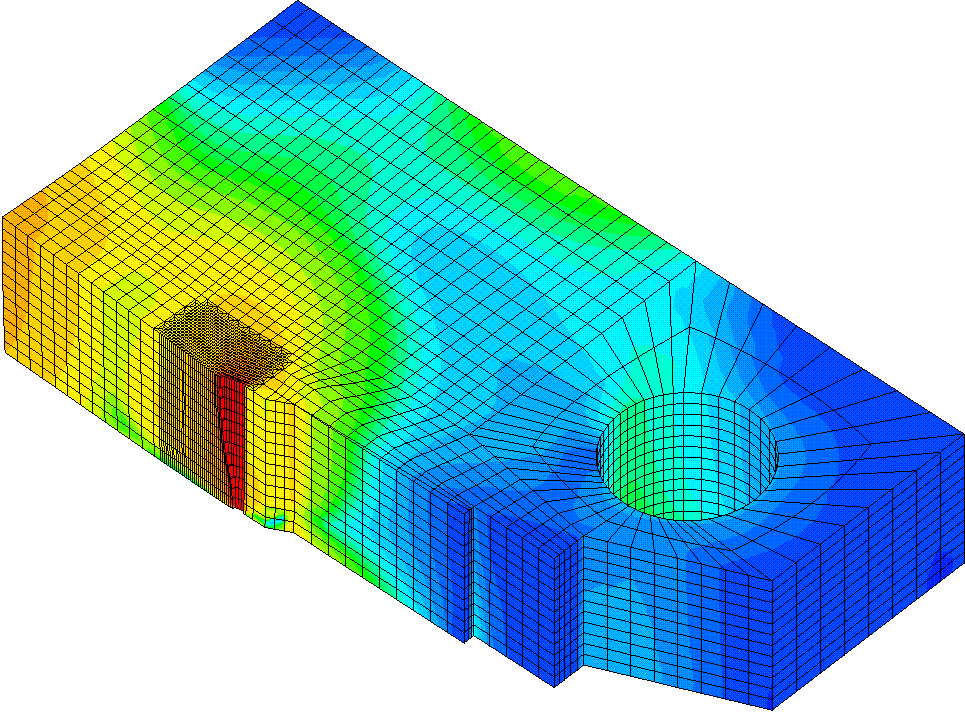
\includegraphics[height=0.25\textheight]{images/rousselier_04}
        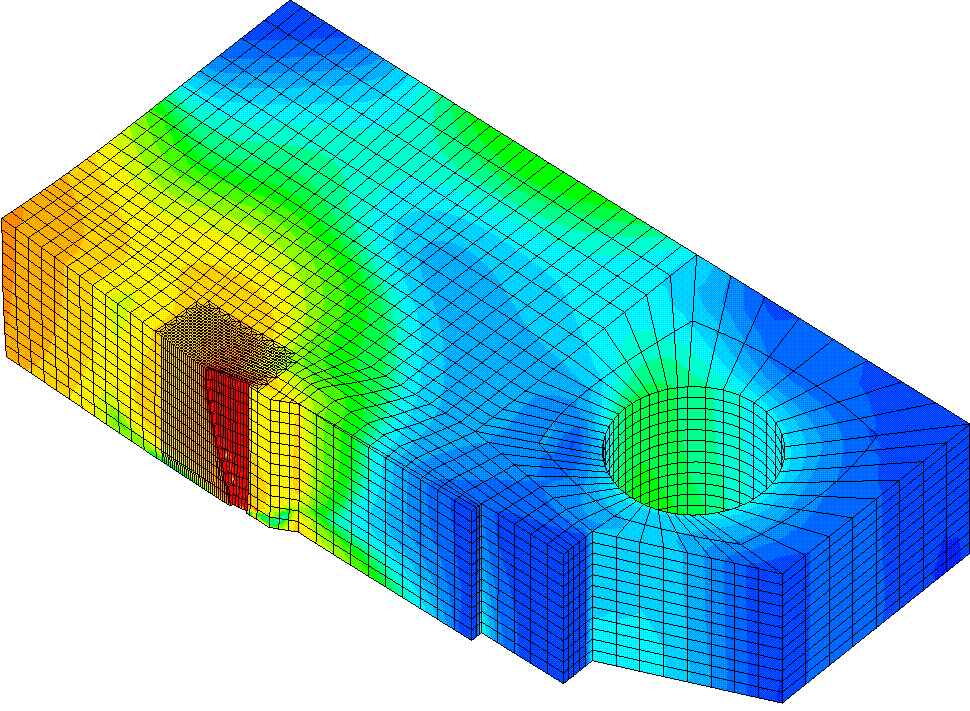
\includegraphics[height=0.25\textheight]{images/rousselier_05}\\
        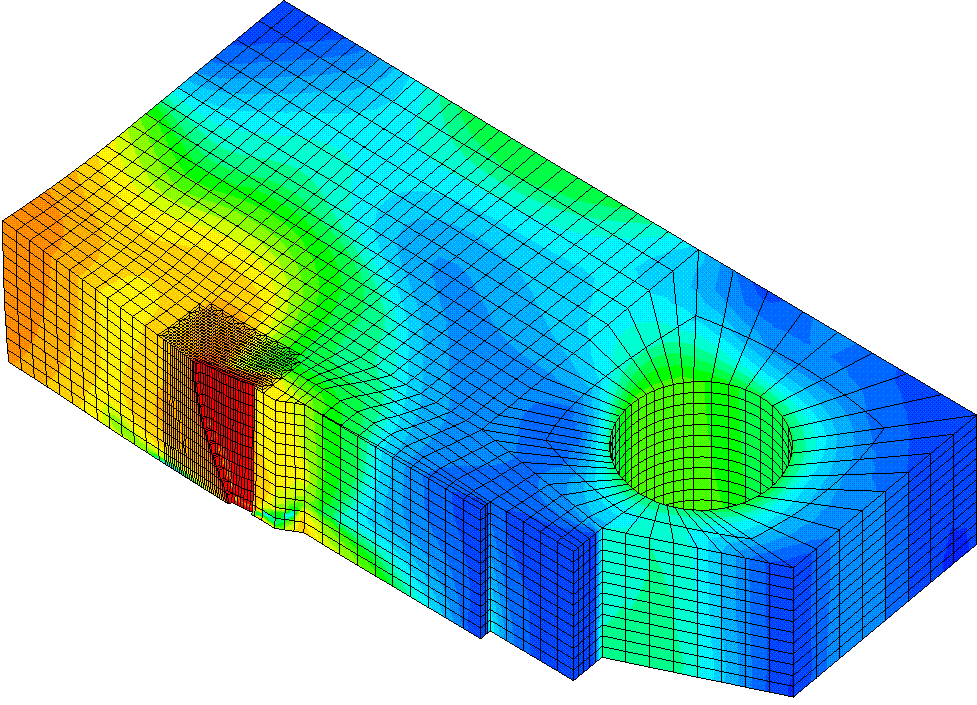
\includegraphics[height=0.25\textheight]{images/rousselier_06}
        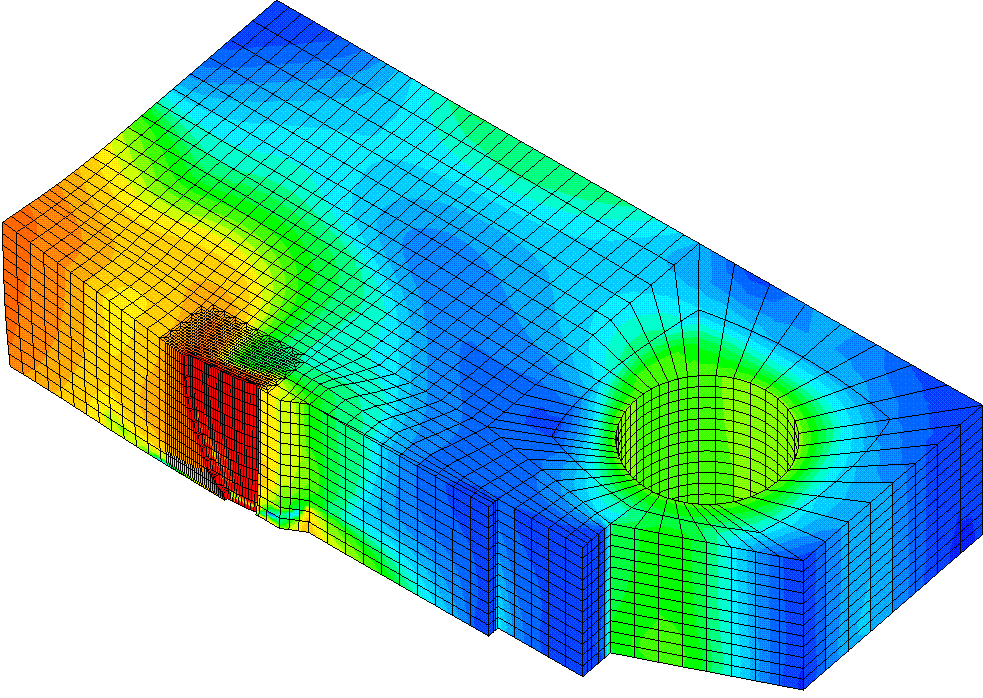
\includegraphics[height=0.25\textheight]{images/rousselier_07}
        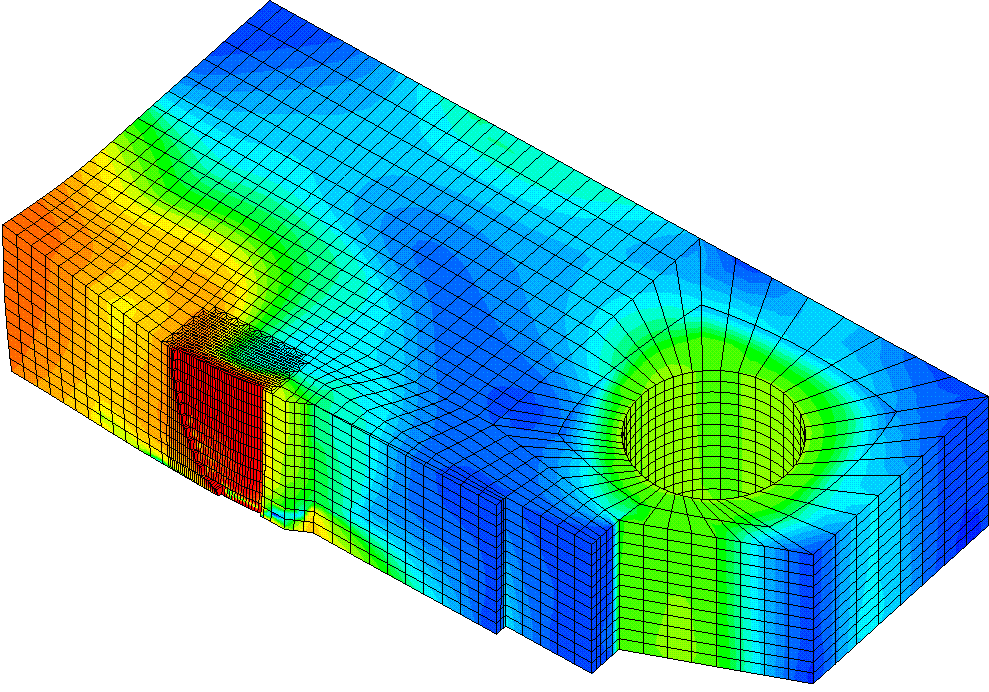
\includegraphics[height=0.25\textheight]{images/rousselier_08}
      \end{textblock*}
      \begin{textblock*}{5cm}(8cm,4.7cm)
        \tiny{\emph{(S. Kebiri)}}
      \end{textblock*}}
    \onslide<5>{
      \begin{textblock*}{12cm}(3.5cm,1.3cm)
        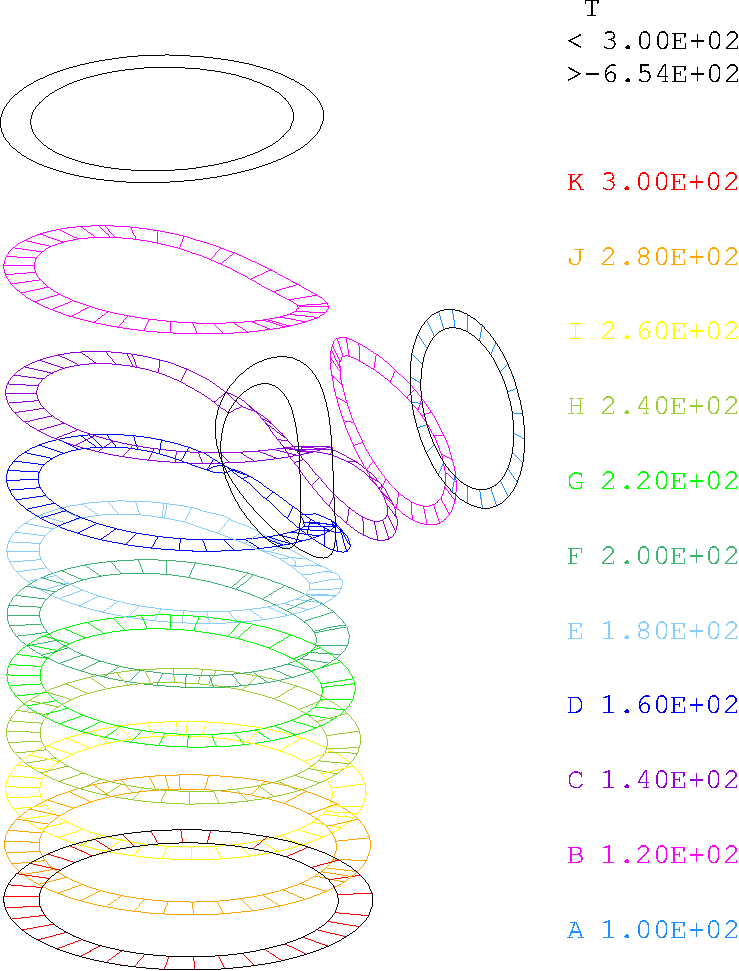
\includegraphics[height=0.4\textheight]{images/te_temperature}\hspace{1cm}
        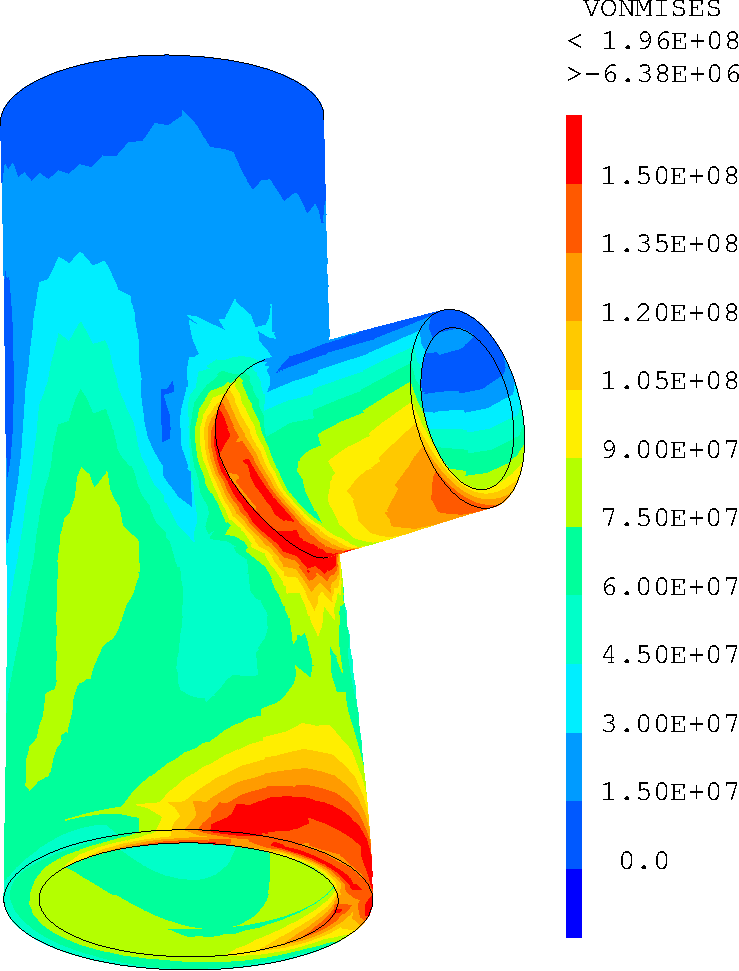
\includegraphics[height=0.4\textheight]{images/te_sigma}
      \end{textblock*}}
    \onslide<6>{
      \begin{textblock*}{12cm}(6.5cm,1.2cm)
        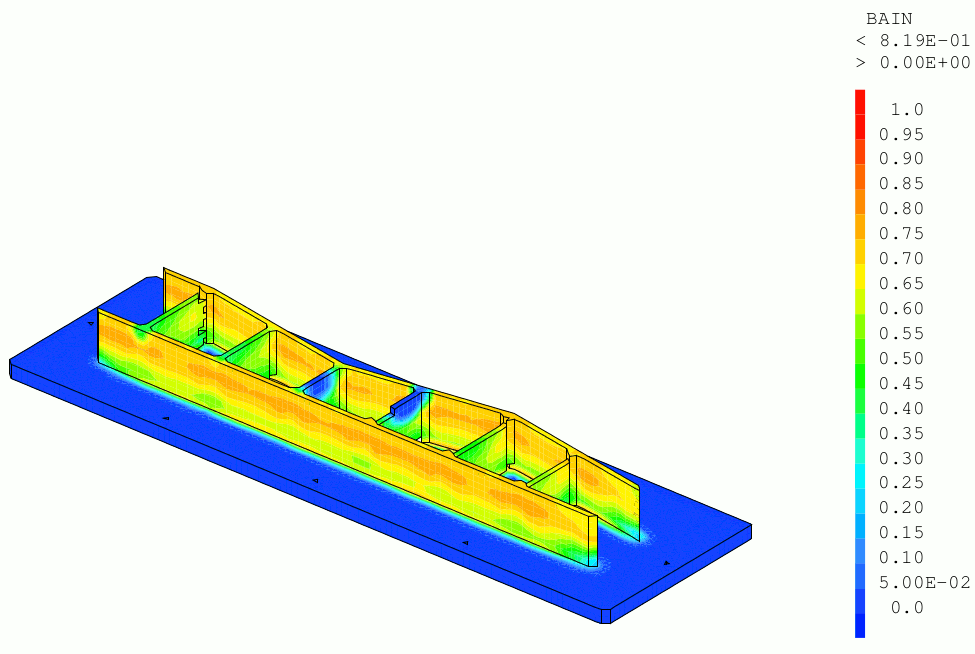
\includegraphics[height=0.4\textheight]{images/metallurgie}
      \end{textblock*}
      \begin{textblock*}{5cm}(8cm,4.7cm)
        \tiny{\emph{(C. Berthinier)}}
      \end{textblock*}}}
    \item<5->\fe{\g{Thermique}}{\g{Thermal analysis}}\\
    \footnotesize{
      \fe{Conduction, convection, rayonnement, changement de phase}
       {Conduction, convection, radiation, phase transition}}
    \item<6->\fe{\g{Mécanique des fluides}}{\g{Fluid mechanics}}
    \item<6->\fe{\g{Diffusion} multi espèces (loi de Fick)}{Multi species \g{diffusion} (Fick's law)}
    \item<6->\fe{Magnétostatique}{Magneto-statics}
    \item<6->\fe{Métallurgie}{Metallurgy}
    \item<6->\fe{Couplage thermo-hygro-mécanique}{Thermo-hygro-mechanics coupling}
  \end{itemize}}
\end{frame}

\begin{frame}{\fe{Présentation de PASAPAS}{The PASAPAS procedure}}
  \begin{itemize}
    \item \fe{Objectif}{Objective}\\
    \footnotesize
    \fe{Résolution de problèmes \emph{non linéaires évolutifs} de manière incrémentale\\
        en \red{thermique} et en \blue{mécanique}\\
        le temps peut être physique (ex~: thermique transitoire)\\
        ou non (ex~: plasticité avec chargement progressif)\\
        $\rightarrow$ on parle donc volontiers de \emph{variable d'évolution}\\}
       {Incremental solving of \emph{non linear progressive}\\
        \red{thermal} and \blue{mechanical} problems\\
        Time can be physical (e.g. thermal transients)\\
        or not (e.g. plasticity with progressive loading)\\
        $\rightarrow$ time or pseudo-time is called the \emph{evolution parameter}\\}
    ~
    \normalsize
    \item \fe{Types de non linéarités traitées}{Non linear phenomena considered}\\
    \fe{\red{Comportement} \footnotesize (plasticité, endommagement, matériaux variables, etc.) \normalsize\\
        \orange{Géométrie} \footnotesize (grands déplacements) \normalsize\\
        \green{Déformations} \footnotesize (grandes rotations) \normalsize\\
        \violet{Conditions limites} \footnotesize (rayonnement, frottement, pression suiveuse, etc.) \normalsize}
       {\red{Behavior} (plasticity, damage, variable material properties, etc.)\\
        \orange{Geometry} (large displacements)\\
        \green{Strains} (large rotations)\\
        \violet{Boundary conditions} (radiation, friction, following pressure, etc.)}
  \end{itemize}
\end{frame}

\begin{frame}{\fe{Utilisation de PASAPAS}{PASAPAS use}}
  \begin{itemize}
    \item \fe{\g{Créer une table} contenant toutes les données du problème}
             {\g{Create a table} containing all the data:}\\
    \lstinputlisting[language=gibiane, firstline=1, lastline=9]{dgibi/exemples.dgibi}
    \item \fe{\g{Appeler la procédure}}{\g{Procedure call:}}\\
    \lstinputlisting[language=gibiane, firstline=11, lastline=11]{dgibi/exemples.dgibi}
    \item \fe{\g{Post traitement} des résultats}{Results \g{post-processing}}
  \end{itemize}
\end{frame}

\begin{frame}{\fe{Aperçu des paramètres d'entrée}{Overview of input parameters}}
  \begin{itemize}
    \item \fe{Généralités}{General}\\
    \tiny
    \begin{tabular}{lll}
    \kwg{'MODELE'}           & MMODEL   & \fe{Équations à résoudre, formulation EF (\kwr{MODE})}
                                             {Equations to solve, FE formulation (\kwr{MODE})}\\
    \kwg{'CARACTERISTIQUES'} & MCHAML   & \fe{Paramètres matériau et/ou géométriques (\kwr{MATE})}
                                             {Material and/or geometrical parameters (\kwr{MATE})}\\
    \kwg{'CHARGEMENT'}       & CHARGEME & \fe{Évolution des CL et chargements au cours du calcul (\kwr{CHAR})}
                                             {BC and loading variation during calculation (\kwr{CHAR})}\\
    \end{tabular}
    \normalsize
    \item \fe{Thermique}{Thermal analysis}\\
    \tiny
    \begin{tabular}{lll}
    \kwg{'BLOCAGES\_THERMIQUES'} & RIGIDITE & \fe{Matrice de blocage des CL de type Dirichlet (\kwr{BLOQ,RELA})}
                                                 {Stiffness matrix for Dirichlet BC (\kwr{BLOQ,RELA})}\\
    \kwg{'CELSIUS'}              & LOGIQUE  & \fe{= VRAI si les températures sont en degrés Celsius}
                                                 {=VRAI (true) if temperature unit is Celsius}\\
    \kwg{'TEMPERATURES' . 0}     & CHPOINT  & \fe{Conditions initiales}
                                                 {Initial conditions}\\
    \end{tabular}
    \normalsize
    \item \fe{Mécanique}{Mechanics}\\
    \tiny
    \begin{tabular}{lll}
    \kwg{'BLOCAGES\_MECANIQUES'}           & RIGIDITE & \fe{Matrice de blocage des CL de type Dirichlet (\kwr{BLOQ,RELA})}
                                                           {Stiffness matrix for Dirichlet BC (\kwr{BLOQ,RELA})}\\
    \kwg{'GRANDS\_DEPLACEMENTS'}           & LOGIQUE  & \fe{Équilibre vérifié sur les configurations déformées}
                                                           {Equilibrium checked on the deformed mesh}\\
    \kwg{'DEPLACEMENTS' . 0}               & CHPOINT  & \fe{Conditions initiales}
                                                           {Initial conditions}\\
    \kwg{'CONTRAINTES' . 0}                & MCHAML   & \fe{Idem}{Idem}\\
    \kwg{'VARIABLES\_INTERNES' . 0}        & MCHAML   & \fe{Idem}{Idem}\\
    \kwg{'DEFORMATIONS\_INELASTIQUES' . 0} & MCHAML   & \fe{Idem}{Idem}\\
    \end{tabular}
    \normalsize
    \item \fe{Mécanique (dynamique)}{Mechanics (dynamics)}\\
    \tiny
    \begin{tabular}{lll}
    \kwg{'DYNAMIQUE'}          & LOGIQUE  & \fe{= VRAI si calcul dynamique}
                                               {= VRAI (true) for dynamics calculations}\\
    \kwg{'AMORTISSEMENT'}      & RIGIDITE & \fe{Matrice d'amortissement}
                                               {Damping matrix}\\
    \kwg{'VITESSES' . 0}       & MCHAML   & \fe{Conditions initiales}
                                               {Initial conditions}\\
    \kwg{'ACCELERATIONS' . 0 } & CHPOINT  & Idem\\
    \end{tabular}
    \normalsize
    \item \fe{Instants de calcul et sauvegarde}{Calculation and saving times}\\
    \tiny
    \begin{tabular}{lll}
    \kwg{'TEMPS\_CALCULES'} & LISTREEL & \fe{Liste des instants de calcul (\kwr{PROG})}
                                            {List of times for which results are computed (\kwr{PROG})}\\
    \kwg{'TEMPS\_SAUVES'}   & LISTREEL & \fe{Liste des instants pour lesquels les résultats sont conservés (\kwr{PROG})}
                                            {List of times for which results are saved (\kwr{PROG})}\\
    \end{tabular}
    \normalsize
  \end{itemize}
\end{frame}

\begin{frame}{\fe{Aperçu des paramètres de sortie}{Overview of ouput parameters}}
  \begin{itemize}
    \item \fe{Résultats}{Results}\\
    \tiny
    \begin{tabular}{lll}
    \kwg{'TEMPS'}                      & TABLE & \fe{Instants de calcul, identiques aux \kwg{'TEMPS\_SAUVES'}}
                                                    {Time values, identical to \kwg{'TEMPS\_SAUVES'}}\\
    & & \\
    \kwg{'TEMPERATURES'}               & TABLE & \fe{Champs solutions pour chaque \kwg{'TEMPS\_SAUVES'}}
                                                    {Fields (solution) calculated for each stored time \kwg{'TEMPS\_SAUVES'}}\\
    \kwg{'PROPORTION\_PHASE'}          & TABLE & \fe{Idem}{Idem}\\
    & & \\
    \kwg{'DEPLACEMENTS'}               & TABLE & \fe{Idem}{Idem}\\
    \kwg{'REACTIONS'}                  & TABLE & \fe{Idem}{Idem}\\
    \kwg{'CONTRAINTES'}                & TABLE & \fe{Idem}{Idem}\\
    \kwg{'DEFORMATIONS\_INELASTIQUES'} & TABLE & \fe{Idem}{Idem}\\
    \kwg{'VARIABLES\_INTERNES'}        & TABLE & \fe{Idem}{Idem}\\
    \kwg{'VITESSES'}                   & TABLE & \fe{Idem}{Idem}\\
    \kwg{'ACCELERATIONS'}              & TABLE & \fe{Idem}{Idem}\\
    \end{tabular}
    \normalsize
  \end{itemize}
\end{frame}

\begin{frame}{\fe{Exemples de post traitement}{Post processing examples}}
  \begin{itemize}
    \item \fe{Extraction des champs solution :}{Solution fields extraction:}\\
      \fe{avec l'indice dans la table}{from the table index}\\
      \lstinputlisting[language=gibiane, firstline=13, lastline=13]{dgibi/exemples.dgibi}
      \fe{ou bien avec l'instant de calcul}{or from the time value}\\
      \lstinputlisting[language=gibiane, firstline=14, lastline=14]{dgibi/exemples.dgibi}
    \item \fe{Tracé en mode graphique interactif :}{Graphical mode, interactive plot:}\\
    \lstinputlisting[language=gibiane, firstline=15, lastline=15]{dgibi/exemples.dgibi}
    \item \fe{Évolution temporelle d'un champ calculé :}{Evolution of calculated field with time:}\\
    \lstinputlisting[language=gibiane, firstline=16, lastline=16]{dgibi/exemples.dgibi}
  \end{itemize}
\end{frame}
